\section{Modeling}\label{sec:modeling}
One of the most pressing questions related to this work is whether or not the
increased star-to-star variability in the activity metric and the Jao Gap,
which are coincident in magnitude, are driven by the same underlying mechanism.
The challenge when addressing this question arises from current computational
limitations. Specifically, the kinds of three dimensional
magneto-hydrodynamical simulations --- which would be needed to derive the
effects of convective kissing instabilities on the magnetic field of the star
--- are infeasible to run over gigayear timescales while maintaining thermal
timescale resolutions needed to resolve periodic mixing events.

In order to address this and answer the specific question of \textit{could
kissing instabilities result in increased star-to-star variability of the
magnetic field}, we adopt a very simple toy model. Kissing instabilities result
in a transient radiative zone separating the core of a star (convective) from its
envelope (convective). When this radiative zone breaks down two important
things happen: one, the entire star becomes mechanically coupled, and two,
convective currents can now move over the entire radius of the star.
\citet{Jao2023} propose that this mechanical coupling may allow the star's core
to act as an angular momentum sink thus accelerating a stars spin down and
resulting in anomalously low H$\alpha$ emission. 

Regardless of the exact mechanism by which the magnetic field may be affected,
it is reasonable to expect that both the mechanical coupling and the change to
the scale of convective currents will have some effect on the star's magnetic
field. On a microscopic scale both of these will change how packets of charge
within a star move and may serve to disrupt a stable dynamo. Therefore, in the
model we present here we make only one primary assumption: \textit{every mixing
event may modify the star's magnetic field by some amount}. Within our model
this assumption manifests as a random linear perturbation applied to some base
magnetic field at every mixing event. The strength of this perturbation is 
sampled from a normal distribution with some standard deviation, $\sigma_{B}$.

Synthetic stars are sampled from a grid of stellar models evolved using the
Dartmouth Stellar Evolution Program (DSEP) with similar parameters to those
used in \citet{Boudreaux2023}. Each stellar model was evolved using a high
temporal resolution (timesteps no larger than 10,000 years) and typical
numerical tolerances of one part in $10^5$. Each model was based on a GS98
\citep{Grevesse1998} solar composition with a mass range from 0.3 M$_{\odot}$
to 0.4 M$_{\odot}$. Finally, models adopt OPLIB high temperature radiative
opacities, Ferguson 2004 low temperature radiative opacities, and include both
atomic diffusion and gravitational settling. A Kippenhan-Iben diagram showing
the structural evolution of a model within the Gap is shown in Figure
\ref{fig:kippenhan}.

\begin{figure*}
  \centering
  \includegraphics[width=0.9\textwidth]{Kippenhan_clamped.pdf}
  \caption{Kippenhan-Iben diagram for a 0.345 solar mass star. Note the
  periodic mixing events (where the plotted curves peak).}
  \label{fig:kippenhan}
\end{figure*}

Each synthetic star is assigned some base magnetic activity ($B_{0} \sim
\mathcal{N}(1, \sigma_{B})$) and then the number of mixing events before some age $t$
are counted based on local maxima in the core temperature. The toy magnetic
activity at age $t$ for the model is given in Equation \ref{eqn:activity}. An
example of the magnetic evolution resulting from this model is given in Figure
\ref{fig:simpleB}. Fundamentally, this model presents magnetic
activity variation due to mixing events as a random walk and therefore results will
increasing divergence over time.

\begin{align}\label{eqn:activity}
  B(t) = B_{0} + \sum_{i}B_{i} \sim \mathcal{N}(1, \sigma_{B}) 
\end{align}

\begin{figure}
  \centering
  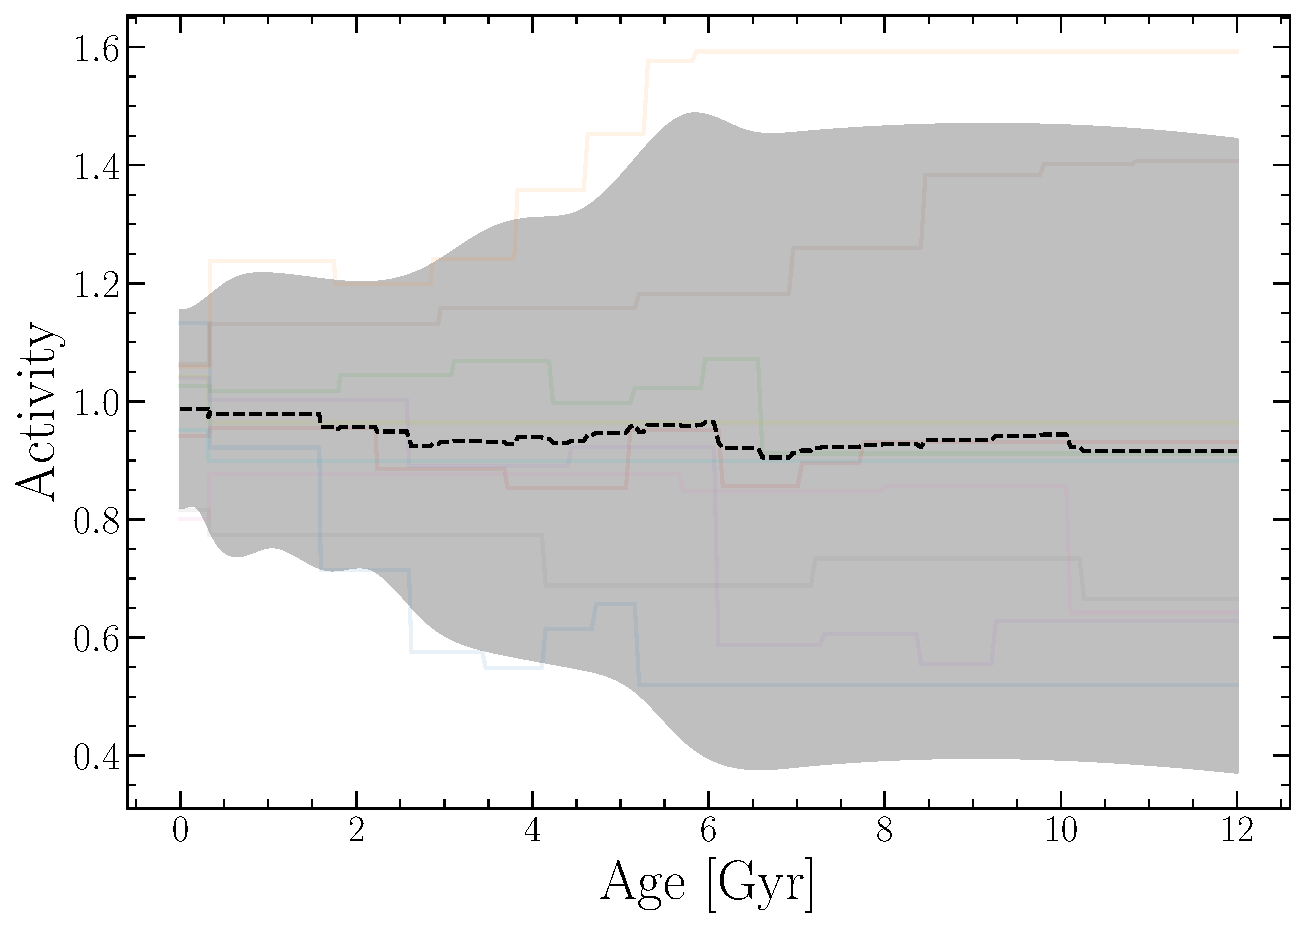
\includegraphics[width=0.45\textwidth]{simpleBEvolution.pdf}
  \caption{Example of the toy model presented here resulting in increased
  divergence between stars magnetic fields. The shaded region represents the
  maximum spread in the two point correlation function at each age.}
  \label{fig:simpleB}
\end{figure}

Applying the same analysis to these models as was done to the observations as
described in Section \ref{sec:results} we find that this simple model results
in a qualitatively similar trend in the standard deviation vs. Magnitude graph
(Figure \ref{fig:model}). In order to reproduce the approximately 50 percent
change to the spread of the activity metric observed in the combined dataset in
section \ref{sec:results} a distribution with a standard deviation of 0.1 is
required when sampling the change in the magnetic activity metric at each
mixing event. This corresponds to 68 percent of mixing events modifying the
activity strength by 10 percent or less. The interpretation here is important:
what this qualitative similarity demonstrates is that it may be reasonable to
expect kissing instabilities to result in the observed increased star-to-star
variation. Importantly, we are not able to claim that kissing instabilities
\textit{do} lead to these increased variations, only that they reasonably
could. Further modeling, observational, and theoretical efforts will be needed
to more definitively answer this question.

\begin{figure}
  \centering
  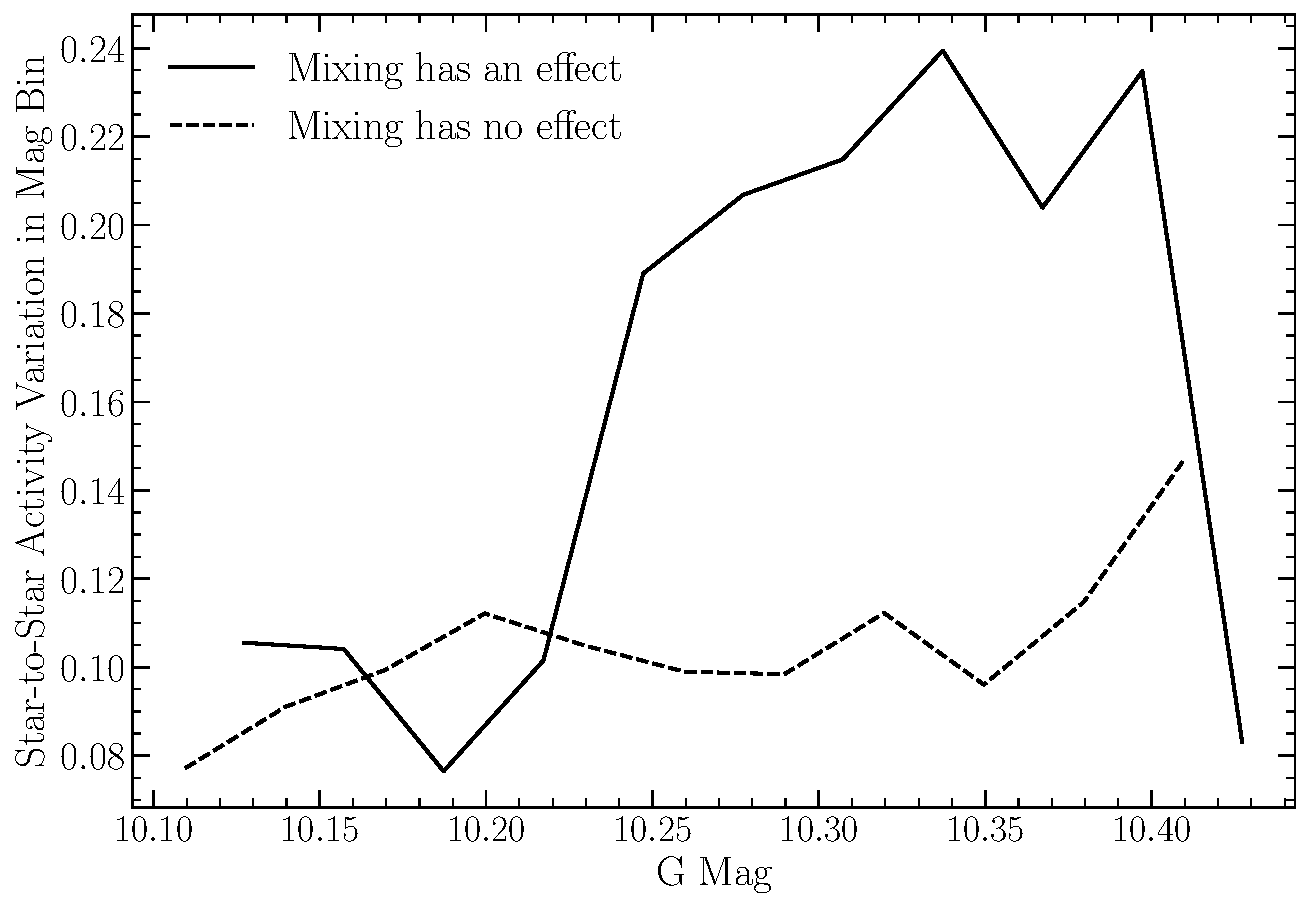
\includegraphics[width=0.45\textwidth]{SpreadModel.pdf}
  \caption{Toy model results showing a qualitatively similar discontinuity in the star-to-star magnetic activity variability.}
  \label{fig:model}
\end{figure}

\subsection{Limitations}
The model presented in this paper is very limited and it is important to keep
these limitations in mind when interpreting the results presented here. Some of
the main challenges which should be leveled at this model are the assumption
that the magnetic field will be altered by some small random perturbation at
every mixing event. This assumption was informed by the large number of free
parameters available to a physical star during the establishment of a large
scale magnetic field and the associated likely stochastic nature of that
process. However, it is similarly believable that the magnetic field will tend
to alter in a uniform manner at each mixing event. For example, since
differential rotation is generally proportional to the temperature gradient
within a star and activity is strongly coupled to differential rotation then it
may be that as the radiative zone reforms over thermal timescales the
homogenization of angular momentum throughout the star results in overall lower
amounts of differential rotation each after mixing event than would otherwise
be present.

Moreover, this model does not consider how other degenerate sources of magnetic
evolution such as stellar spin down, relaxation, or coronal heating may effect
star-to-star variability. These could conceivably lead to a similar increase in
star-to-star variability which is coincident with the Jao Gap magnitude as the
switch from fully to partially convective may effect efficiency of these
process.

Additionally, there are challenges with this toy model that originate from the
stellar evolutionary model. Observations of the Jao Gap show that the feature
is not perpendicular to the magnitude axis; rather, it is inversely
proportional to the color. No models of the Jao Gap published at the time of
writing capture this color dependency and \textit{what causes this color
dependency} remains one of the most pressing questions relating to the
underlying physics. This non captured physics is one potential explanation for
why the magnitude where our model predicts the increase in variability is not
in agreement with where the variability jump exists in the data.

Finally, we have not considered detailed descriptions of the dynamos of stars.
The magnetohydrodynamical modeling which would be required to model the
evolution of the magnetic field of these stars at thermal timescale resolutions
over gigayears is currently beyond the ability of practical computing.
Therefore future work should focus on limited modeling which may inform the
evolution of the magnetic field directly around the time of a mixing event.
